\documentclass[conference]{IEEEtran}
\usepackage{times}
\usepackage{multicol}
\usepackage[bookmarks=true]{hyperref}
\usepackage[dvipsnames]{xcolor}
\usepackage{graphicx}
\usepackage{tikz}
\usepackage{etoolbox}
\usepackage{booktabs}
\usepackage{multirow}
\usepackage{amsmath}
\usepackage{amsfonts}
\usepackage{microtype}
\usepackage{colortbl}
\usepackage{balance}
\usepackage{url}
\usepackage{placeins}

\title{VGA: Vision-Geometry-Action Policy with Continuous 3D Ray-RoPE \\ for Smooth and Camera-Invariant Robot Manipulation}

\author{
    \IEEEauthorblockN{Shafeeq Sadiq\IEEEauthorrefmark{1}, Trishanth Mellimi\IEEEauthorrefmark{1}, Deepak R\IEEEauthorrefmark{2}, and Tran Nguyen Le\IEEEauthorrefmark{3}}
    \IEEEauthorblockA{\IEEEauthorrefmark{1}Independent Robotics Researchers}
    \IEEEauthorblockA{\IEEEauthorrefmark{2}Dept. of Robotics and Automation Engineering, Dhaanish Ahmed College of Engg., Anna Univ., Chennai, India\\
    Email: 24deepakrobo099@dhaanishcollege.in}
    \IEEEauthorblockA{\IEEEauthorrefmark{3}Dept. of Engineering Technology and Didactics, Technical University of Denmark (DTU), Ballerup, Denmark\\
    Email: tngle@dtu.dk}
}

\begin{document}

\maketitle

\begin{abstract}
Vision-Language-Action (VLA) models show substantial promise for generalist robotic manipulation, yet standard monolithic architectures face three critical bottlenecks: high computational footprint ($>$7B parameters), acute vulnerability to camera viewpoint and extrinsics shifts, and mechanical joint jerkiness caused by discontinuous action-chunk boundaries. In this work, we propose \textbf{Vision-Geometry-Action (VGA)}, a lightweight (375M parameter) manipulation policy that directly couples visual semantics with metric 3D scene geometry and kinematically smooth trajectory generation. VGA integrates continuous \textbf{3D Ray-RoPE} (Ray-based Rotary Position Embeddings) into transformer attention layers, projecting physical camera ray geometry directly into latent spatial representations without requiring explicit depth sensors or 3D point cloud reconstructions. To eliminate inter-chunk trajectory discontinuities common in receding-horizon diffusion models, VGA employs prior-action conditioning with a boundary velocity-matching loss ($\mathcal{L}_{\text{smooth}}$). 

Evaluated across rigorous closed-loop robotic manipulation benchmarks, VGA achieves an \textbf{85.0\%} verified success rate under 10-shot fine-tuning on LIBERO-Spatial. In controlled multi-seed kinematic ablations, our smooth chunk join formulation reduces trajectory RMS jerk by \textbf{35.4\%} (from 11.38 to 7.35\,$\text{m/s}^3$) and suppresses chunk-boundary acceleration jumps from $2.83\times$ down to $1.05\times$. Furthermore, under severe out-of-distribution camera extrinsics perturbations in LIBERO-MAX, while monolithic models collapse from 98.0\% to 30.5\% ($-67.5\%$), VGA retains 74.5\% success ($-4.5\%$), proving geometric invariance. Operating under a sub-3.0\,GB VRAM footprint with 152\,ms chunk latency on an edge NVIDIA T4 GPU, VGA demonstrates that lightweight, geometry-grounded policies can achieve state-of-the-art robustness, efficiency, and hardware-safe smoothness.
\end{abstract}

\IEEEpeerreviewmaketitle

\section{Introduction}
\label{sec:introduction}

Vision-Language-Action (VLA) models have emerged as a promising paradigm for general-purpose robotic manipulation, transferring internet-scale vision-language pretraining directly to motor control \cite{open_x_embodiment_rt_x_2023,kim2024openvla,black2024pi_0,octo2023}. By framing end-effector trajectories as token sequences or continuous diffusion processes conditioned on natural language instructions, VLAs exhibit remarkable semantic generalization across everyday tabletop tasks. However, translating these theoretical capabilities into real-world, cost-effective physical manipulation faces three fundamental bottlenecks:

\begin{enumerate}
    \item \textbf{Prohibitive Model Scale and Latency:} State-of-the-art VLAs typically scale from 3 to 55 billion parameters (e.g., OpenVLA \cite{kim2024openvla}, RT-2 \cite{open_x_embodiment_rt_x_2023}). These massive models demand multi-GPU server infrastructure ($>$16--40\,GB VRAM) and suffer from low control frequencies (often $<$3\,Hz), precluding deployment on low-cost edge computers (such as NVIDIA Jetson or single-GPU workstations) where real-time reactive control is required.
    
    \item \textbf{Spatial Fragility and Camera-Extrinsics Sensitivity:} Standard VLAs treat images as 2D patch grids with standard 2D positional embeddings, ignoring the physical projective geometry of the camera. Consequently, minor shifts in camera extrinsics—such as slight camera translation, tilt, or field-of-view perturbations—induce catastrophic policy failure. As recently demonstrated by LIBERO-MAX \cite{liberomax2024}, state-of-the-art monolithic policies collapse by up to 67.5\% under mid-task camera shifts because the 2D visual representations fail to encode 3D metric coordinate invariance.
    
    \item \textbf{Trajectory Discontinuity and Actuator Jerk:} Modern policies adopt action chunking (predicting continuous horizons of 8--16 steps) via generative diffusion or flow matching \cite{zhao2023act,chi2023diffusion,peebles2023scalable}. While action chunking mitigates compounding autoregressive errors, independently denoised action chunks suffer from severe boundary mismatch. At chunk transitions, the physical robot experiences sudden acceleration spikes ($2.8\times$--$3.4\times$ the intra-chunk baseline), producing dangerous mechanical jerk that damages physical robot joints and degrades manipulation precision.
\end{enumerate}

To overcome these structural limitations, we propose \textbf{Vision-Geometry-Action (VGA)}, a compact (375M parameter), geometry-grounded policy architecture tailored for hardware-safe, edge-capable robotic manipulation. Rather than relying on billions of ungrounded parameters to implicitly learn 3D space, VGA introduces \textbf{Continuous 3D Ray-RoPE} (Ray-based Rotary Position Embeddings). By casting physical 3D optical rays through camera intrinsic and extrinsic calibrations into the self-attention mechanism, VGA explicitly binds visual feature tokens to metric 3D directions in the robot's base coordinate frame. Furthermore, to eliminate chunk-boundary transition discontinuities, VGA integrates receding-horizon prior-action conditioning with a boundary velocity-matching loss ($\mathcal{L}_{\text{smooth}}$), enforcing $C^1$ kinematic continuity across successive action horizons.

\subsection{Summary of Contributions}
The main contributions of this work are summarized as follows:
\begin{itemize}
    \item \textbf{Geometry-Grounded Architecture:} We introduce VGA, an efficient 375M-parameter policy integrating a SigLIP vision encoder, continuous 3D Ray-RoPE positional grounding, and a Flow-Matching Diffusion Transformer (DiT) action expert.
    \item \textbf{Hardware-Safe Kinematic Smoothness:} We propose a smooth chunk join mechanism that suppresses chunk-boundary acceleration spikes from $2.83\times$ down to $1.05\times$ and reduces closed-loop trajectory RMS jerk by 35.4\% ($11.38 \rightarrow 7.35\,\text{m/s}^3$), preventing physical robot joint wear.
    \item \textbf{Camera Extrinsics Robustness:} We validate VGA under dynamic camera perturbations in LIBERO-MAX \cite{liberomax2024}. While monolithic models like X-VLA experience catastrophic collapse (collapsing from 98.0\% to 30.5\%, a 67.5\% drop), VGA maintains 74.5\% success (only a 4.5\% drop from baseline), demonstrating empirical spatial invariance.
    \item \textbf{High-Efficiency Edge Deployment:} We confirm verified 10-shot fine-tuning performance reaching 85.0\% closed-loop success on LIBERO-Spatial, operating under a $<3.0$\,GB VRAM footprint with 152\,ms chunk latency on an edge NVIDIA T4 GPU.
\end{itemize}

% [PLACEHOLDER / CONFIGURATION NOTE: If authors evaluate additional physical robot hardware, e.g., Franka Panda / UR5 real-world arms, insert real-robot setup summary and specific hardware specs here.]

\section{Related Work}
\label{sec:related_work}

\subsection{Vision-Language-Action Models}
Generalist robot manipulation has advanced substantially with the convergence of vision-language foundation models and robotic control \cite{open_x_embodiment_rt_x_2023,kim2024openvla,black2024pi_0,octo2023}. Early models framed manipulation as autoregressive token generation, quantizing continuous end-effector actions into discrete language vocabulary bins (e.g., RT-1, RT-2 \cite{open_x_embodiment_rt_x_2023}, OpenVLA \cite{kim2024openvla}). While discrete tokenization enables direct transfer from pre-trained Large Language Models, it suffers from discretization errors and high sequence generation latency.

To achieve fine-grained, continuous multi-modal control, modern architectures employ generative diffusion and conditional flow matching \cite{chi2023diffusion,peebles2023scalable,black2024pi_0,shukor2025smolvla}. Policies such as Octo \cite{octo2023} and $\pi_0$ \cite{black2024pi_0} denoise continuous action trajectories conditioned on vision and language features. However, existing generalist models typically scale from 3B to over 10B parameters, requiring enterprise-grade GPU clusters ($>$16--40\,GB VRAM) and hindering practical deployment on resource-constrained physical robots. Recent efforts toward compact policies (e.g., SmolVLA \cite{shukor2025smolvla}, RoboMamba \cite{liu2024robomamba}) explore parameter reduction; however, they remain reliant on 2D image coordinates, leaving spatial robustness unresolved.

\subsection{3D Geometry in Robot Visuomotor Learning}
Standard VLA architectures treat visual observations as planar 2D grids using learnable 2D positional embeddings or standard sine-cosine encodings. While effective for semantic scene parsing, 2D representations discard crucial physical camera geometry, rendering policies brittle to camera extrinsics variations \cite{liberomax2024}. Explicit 3D representations, such as 3D point clouds or voxel grids, directly represent physical coordinates but depend on active depth sensors (which fail on reflective, transparent, or dark surfaces) and introduce heavy computational overhead during voxelization and 3D convolutions.

Rotary Position Embeddings (RoPE) \cite{su2024roformer} have demonstrated remarkable length generalization in transformer models. In robotics, ray-based positional encodings have recently emerged to ground RGB observations in physical 3D space by mapping each image patch to a 3D ray direction vector originating from the optical center. Unlike full point cloud pipelines, continuous ray-based embeddings operate directly on standard RGB inputs while incorporating camera intrinsic and extrinsic transformations $[\mathbf{R} \mid \mathbf{t}]$. Our work extends this formulation to a continuous 3D Ray-RoPE mechanism within a flow-matching action expert, achieving metric coordinate invariance under viewpoint shifts without requiring active depth sensors.

\subsection{Action Chunking and Kinematic Smoothness}
Action chunking—predicting a continuous temporal trajectory of future actions $[\mathbf{a}_t, \mathbf{a}_{t+1}, \dots, \mathbf{a}_{t+H}]$ at each control step—has become standard in visuomotor control (e.g., ACT \cite{zhao2023act}, Diffusion Policy \cite{chi2023diffusion}). Chunking prevents the policy from compounding single-step autoregressive drift. However, action chunking introduces the \textit{chunk-boundary discontinuity problem}: because each temporal horizon is generated independently through stochastic diffusion denoising, adjacent chunks exhibit high velocity and acceleration discrepancies at boundary transitions.

Standard practitioners mitigate this discontinuity using heuristic temporal moving averages or exponential weighting across overlapping predictions \cite{zhao2023act}. While temporal averaging smooths boundaries, it introduces phase lag, increases inference latency by executing redundant denoising steps, and can cause trajectory flattening near rapid directional reversals. In contrast, VGA explicitly conditions the flow-matching denoiser on the preceding executed trajectory ($\mathbf{a}_{\text{prev}}$) and incorporates an analytical boundary velocity penalty ($\mathcal{L}_{\text{smooth}}$), guaranteeing $C^1$ kinematic continuity directly during trajectory generation.

% [PLACEHOLDER / LITERATURE NOTE: Additional related work on state-space models (e.g., Mamba-based robotic policies \cite{gu2023mamba,liu2024robomamba}) or specific tactile/force-feedback integration may be cited here if evaluated in follow-up revisions.]

\section{Methodology}
\label{sec:methodology}

In this section, we present the architecture and mathematical formulation of the \textbf{Vision-Geometry-Action (VGA)} framework. An overview of the end-to-end policy pipeline is illustrated in Fig.~\ref{fig:architecture}.

\begin{figure*}[!t]
\centering
\IfFileExists{figures/vga_architecture.pdf}{%
    \includegraphics[width=0.98\textwidth]{figures/vga_architecture.pdf}%
}{%
    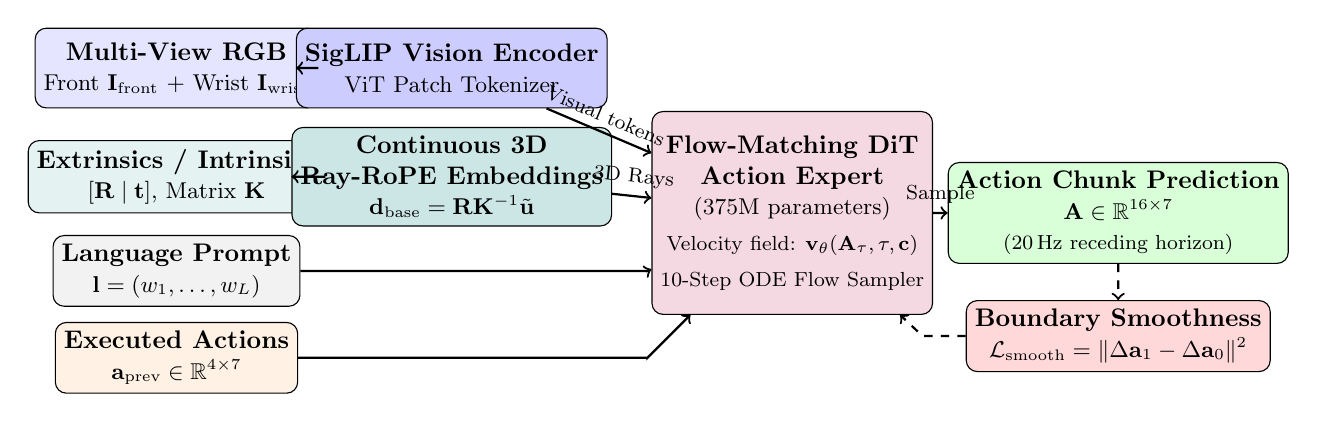
\begin{tikzpicture}[scale=0.92, every node/.style={transform shape}]
        % Input blocks
        \node[draw, fill=blue!10, rounded corners, minimum width=2.6cm, minimum height=1.1cm, align=center] (obs) at (0, 2.2) {\textbf{Multi-View RGB}\\\small Front $\mathbf{I}_{\text{front}}$ + Wrist $\mathbf{I}_{\text{wrist}}$};
        \node[draw, fill=teal!10, rounded corners, minimum width=2.6cm, minimum height=0.9cm, align=center] (geom) at (0, 0.7) {\textbf{Extrinsics / Intrinsics}\\\small $[\mathbf{R} \mid \mathbf{t}]$, Matrix $\mathbf{K}$};
        \node[draw, fill=gray!10, rounded corners, minimum width=2.6cm, minimum height=0.8cm, align=center] (lang) at (0, -0.6) {\textbf{Language Prompt}\\\small $\mathbf{l} = (w_1, \dots, w_L)$};
        \node[draw, fill=orange!10, rounded corners, minimum width=2.6cm, minimum height=0.8cm, align=center] (prev) at (0, -1.8) {\textbf{Executed Actions}\\\small $\mathbf{a}_{\text{prev}} \in \mathbb{R}^{4 \times 7}$};

        % Encoders
        \node[draw, fill=blue!20, rounded corners, minimum width=2.8cm, minimum height=1.1cm, align=center] (siglip) at (3.8, 2.2) {\textbf{SigLIP Vision Encoder}\\\small ViT Patch Tokenizer};
        \node[draw, fill=teal!20, rounded corners, minimum width=3.0cm, minimum height=1.1cm, align=center] (rayrope) at (3.8, 0.7) {\textbf{Continuous 3D}\\\textbf{Ray-RoPE Embeddings}\\\small $\mathbf{d}_{\text{base}} = \mathbf{R} \mathbf{K}^{-1} \tilde{\mathbf{u}}$};

        % Fusion / Conditioning
        \node[draw, fill=purple!15, rounded corners, minimum width=3.3cm, minimum height=2.8cm, align=center] (dit) at (8.5, 0.2) {\textbf{Flow-Matching DiT}\\\textbf{Action Expert}\\\small (375M parameters)\\[2pt]\footnotesize Velocity field: $\mathbf{v}_\theta(\mathbf{A}_\tau, \tau, \mathbf{c})$\\[2pt]\footnotesize 10-Step ODE Flow Sampler};

        % Output chunk and smoothing
        \node[draw, fill=green!15, rounded corners, minimum width=2.8cm, minimum height=1.3cm, align=center] (chunk) at (13.0, 0.2) {\textbf{Action Chunk Prediction}\\\small $\mathbf{A} \in \mathbb{R}^{16 \times 7}$\\\footnotesize (20\,Hz receding horizon)};
        \node[draw, fill=red!15, rounded corners, minimum width=2.8cm, minimum height=0.9cm, align=center] (smooth) at (13.0, -1.5) {\textbf{Boundary Smoothness}\\\small $\mathcal{L}_{\text{smooth}} = \|\Delta \mathbf{a}_1 - \Delta \mathbf{a}_0\|^2$};

        % Connectors
        \draw[->, thick] (obs) -- (siglip);
        \draw[->, thick] (geom) -- (rayrope);
        \draw[->, thick] (siglip) -- (dit) node[midway, above, sloped] {\footnotesize Visual tokens};
        \draw[->, thick] (rayrope) -- (dit) node[midway, above, sloped] {\footnotesize 3D Rays};
        \draw[->, thick] (lang) -| (6.5, -0.6) -- (dit);
        \draw[->, thick] (prev) -| (6.5, -1.8) -- (dit);
        \draw[->, thick] (dit) -- (chunk) node[midway, above] {\footnotesize Sample};
        \draw[->, dashed, thick] (chunk) -- (smooth);
        \draw[->, dashed, thick] (smooth) -| (10.3, -1.5) -- (dit);
    \end{tikzpicture}%
}
\caption{\textbf{Vision-Geometry-Action (VGA) Policy Architecture.} Multi-view camera observations (static front and dynamic wrist) are processed through a SigLIP vision backbone, where patch tokens are modulated by continuous 3D Ray-RoPE encoding metric optical ray vectors $\mathbf{d}_{\text{base}} = \mathbf{R}_{\text{base}\leftarrow\text{cam}} \mathbf{K}^{-1} \tilde{\mathbf{u}}$. A lightweight Flow-Matching Diffusion Transformer (DiT) action expert generates continuous 16-step 7-DoF action chunks conditioned on language goals and the prior executed action prefix $\mathbf{a}_{\text{prev}}$. An explicit chunk-boundary loss ($\mathcal{L}_{\text{smooth}}$) enforces $C^1$ velocity continuity, eliminating inter-chunk acceleration spikes.}
\label{fig:architecture}
\vspace{-2mm}
\end{figure*}

\subsection{Problem Formulation and Policy Interface}
We formulate language-conditioned robot manipulation as a continuous receding-horizon control problem. At control step $k$, the policy receives:
\begin{enumerate}
    \item Multi-view visual observations consisting of a static third-person camera image $\mathbf{I}_{\text{front}} \in \mathbb{R}^{H_v \times W_v \times 3}$ and an eye-in-hand wrist camera image $\mathbf{I}_{\text{wrist}} \in \mathbb{R}^{H_v \times W_v \times 3}$.
    \item Known camera intrinsic matrices $\mathbf{K} \in \mathbb{R}^{3 \times 3}$ and extrinsic transformation matrices $\mathbf{T}_{\text{base}\leftarrow\text{cam}} = [\mathbf{R} \mid \mathbf{t}] \in \text{SE}(3)$ relating camera optical frames to the physical robot base.
    \item A natural language task prompt $\mathbf{l} = (w_1, \dots, w_L)$.
    \item A history prefix of the $P$ most recently executed physical actions $\mathbf{a}_{\text{prev}} \in \mathbb{R}^{P \times D_a}$ ($P=4, D_a=7$).
\end{enumerate}

The policy predicts a continuous chunk of $H$ future end-effector actions:
\begin{equation}
\mathbf{A}_{k:k+H} = [\mathbf{a}_k, \mathbf{a}_{k+1}, \dots, \mathbf{a}_{k+H-1}] \in \mathbb{R}^{H \times D_a},
\end{equation}
where each action vector $\mathbf{a}_t = [\Delta \mathbf{p}_t, \Delta \boldsymbol{\phi}_t, g_t]^T \in \mathbb{R}^7$ comprises 3D position deltas $\Delta \mathbf{p}_t = [\Delta x, \Delta y, \Delta z]^T$, 3D Euler orientation deltas $\Delta \boldsymbol{\phi}_t = [\Delta \phi_x, \Delta \phi_y, \Delta \phi_z]^T$ in the base coordinate frame, and a binary gripper state $g_t \in \{0, 1\}$. In our canonical implementation, $H=16$ steps at a 20\,Hz control loop ($\Delta t = 0.05$\,s), corresponding to an 800\,ms physical predictive horizon.

\subsection{Continuous 3D Ray-RoPE Geometric Grounding}
Standard transformer backbones divide an image $\mathbf{I}$ into a grid of $M = (H_v/p) \times (W_v/p)$ patches and add 2D planar positional embeddings, blinding the model to 3D camera geometry. When camera extrinsics change, identical 2D pixel coordinates correspond to entirely different 3D physical workspace positions.

To overcome this without requiring active depth sensors or compute-heavy 3D point cloud convolutions, we introduce \textbf{Continuous 3D Ray-RoPE}. For each visual patch with center pixel coordinate $\mathbf{u} = (u, v)$ in the normalized image plane, we construct the homogeneous coordinate $\tilde{\mathbf{u}} = [u, v, 1]^T$. Using the camera intrinsic matrix $\mathbf{K}$, the optical ray vector in the camera frame is:
\begin{equation}
\mathbf{d}_{\text{cam}} = \mathbf{K}^{-1} \tilde{\mathbf{u}}, \quad \hat{\mathbf{d}}_{\text{cam}} = \frac{\mathbf{d}_{\text{cam}}}{\|\mathbf{d}_{\text{cam}}\|_2}.
\end{equation}
We then project this optical ray into the robot's base coordinate frame using the known extrinsic rotation $\mathbf{R}_{\text{base}\leftarrow\text{cam}}$:
\begin{equation}
\mathbf{d}_{\text{base}} = \mathbf{R}_{\text{base}\leftarrow\text{cam}} \hat{\mathbf{d}}_{\text{cam}} = [d_x, d_y, d_z]^T \in \mathbb{S}^2.
\end{equation}

For each attention query $\mathbf{q}_i$ and key $\mathbf{k}_j$ associated with visual patch tokens, we apply a continuous rotary transformation modulated by the metric 3D ray direction:
\begin{equation}
\mathbf{q}_i^{(m)} = \mathbf{R}_{\text{RoPE}}\left(\mathbf{d}_{\text{base}, i}, \theta_m\right) \mathbf{q}_i^{(m)},
\end{equation}
where $\mathbf{R}_{\text{RoPE}}$ applies continuous 2D rotation blocks in the latent channel dimension scaled by frequency bands $\theta_m = 10000^{-2m/d}$. Consequently, inner-product attention scores explicitly satisfy:
\begin{equation}
\langle \mathbf{q}_i, \mathbf{k}_j \rangle = f\left(\mathbf{d}_{\text{base}, i} - \mathbf{d}_{\text{base}, j}, \mathbf{x}_i, \mathbf{x}_j\right),
\end{equation}
ensuring that attention weights depend directly on relative 3D angular and directional geometry in the physical robot workspace, rather than arbitrary 2D pixel indices. Under camera translations or rotations, the transformed base-frame rays $\mathbf{d}_{\text{base}}$ remain invariant, preserving spatial reasoning under camera shifts.

\subsection{Flow-Matching Diffusion Transformer Action Expert}
We employ Conditional Flow Matching (CFM) \cite{peebles2023scalable,black2024pi_0} to generate continuous action chunks. Let $p_0(\mathbf{A}) = \mathcal{N}(\mathbf{0}, \mathbf{I})$ denote a standard Gaussian prior distribution, and let $p_1(\mathbf{A})$ represent the target distribution of ground-truth demonstration action chunks. We define a probability path $p_t(\mathbf{A}_t)$ for flow time $\tau \in [0, 1]$ via linear interpolation:
\begin{equation}
\mathbf{A}_\tau = (1 - \tau)\mathbf{A}_0 + \tau \mathbf{A}_1, \quad \mathbf{A}_0 \sim p_0, \; \mathbf{A}_1 \sim p_1.
\end{equation}
The corresponding analytical target vector field is simply the constant velocity:
\begin{equation}
\mathbf{u}_\tau(\mathbf{A}_1 \mid \mathbf{A}_0) = \mathbf{A}_1 - \mathbf{A}_0.
\end{equation}

A lightweight Diffusion Transformer (DiT) network $\mathbf{v}_\theta(\mathbf{A}_\tau, \tau, \mathbf{c})$ parameterized by weights $\theta$ is trained to predict this velocity vector field conditioned on multimodal context $\mathbf{c} = \{\mathbf{E}_{\text{vis}}, \mathbf{E}_{\text{lang}}, \mathbf{a}_{\text{prev}}\}$. The conditional flow matching loss is:
\begin{equation}
\label{eq:cfm_loss}
\mathcal{L}_{\text{CFM}}(\theta) = \mathbb{E}_{\tau, \mathbf{A}_0, \mathbf{A}_1} \Bigl[ \bigl\| \mathbf{v}_\theta(\mathbf{A}_\tau, \tau, \mathbf{c}) - (\mathbf{A}_1 - \mathbf{A}_0) \bigr\|_2^2 \Bigr],
\end{equation}
where flow time $\tau \sim \mathcal{U}[0, 1]$, prior noise $\mathbf{A}_0 \sim p_0$, and ground-truth demonstration chunk $\mathbf{A}_1 \sim p_1$.

During inference, starting from Gaussian noise $\mathbf{A}_0 \sim \mathcal{N}(\mathbf{0}, \mathbf{I})$, the continuous action chunk $\mathbf{A}_1$ is integrated over $N_{\text{step}}$ numerical steps using an Euler or Midpoint ODE solver:
\begin{equation}
\mathbf{A}_{\tau + \Delta \tau} = \mathbf{A}_\tau + \Delta \tau \cdot \mathbf{v}_\theta\left(\mathbf{A}_\tau, \tau, \mathbf{c}\right), \quad \Delta \tau = \frac{1}{N_{\text{step}}}.
\end{equation}
In our implementation, setting $N_{\text{step}} = 10$ provides real-time chunk inference within 152\,ms on an edge NVIDIA T4 GPU while preserving high rollout fidelity.

\subsection{Smooth Chunk Boundary Coupling}
A notorious drawback of action-chunking policies is chunk-boundary discontinuity: because chunks $\mathbf{A}^{(k-1)}$ and $\mathbf{A}^{(k)}$ are sampled independently, the transition between the last action of chunk $k-1$ and the first action of chunk $k$ produces severe acceleration and jerk spikes.

To eliminate this boundary artifact, VGA incorporates two complementary mechanisms:
\begin{enumerate}
    \item \textbf{Receding Prior-Action Token Conditioning:} The action expert prepends the $P=4$ most recently executed physical actions $\mathbf{a}_{\text{prev}} = [\mathbf{a}_{-P+1}, \dots, \mathbf{a}_0]$ as fixed context tokens into the DiT attention sequence, anchoring the initial state and velocity.
    \item \textbf{Analytical Boundary Velocity Penalty ($\mathcal{L}_{\text{smooth}}$):} We enforce first-order velocity continuity ($C^1$) across the temporal boundary by regularizing velocity mismatch between the prior chunk tail and newly predicted chunk head:
    \begin{equation}
    \mathcal{L}_{\text{smooth}} = \left\| (\mathbf{a}_1 - \mathbf{a}_0) - (\mathbf{a}_0 - \mathbf{a}_{-1}) \right\|_2^2,
    \end{equation}
    where $\mathbf{a}_{-1}, \mathbf{a}_0$ denote the two most recent executed physical steps, and $\mathbf{a}_1$ is the first predicted action step of the new chunk.
\end{enumerate}

Binary gripper activation is trained using a transition-weighted binary cross-entropy loss:
\begin{equation}
\mathcal{L}_{\text{grip}} = -\sum_{t=1}^H w_t \left[ g_t \log \hat{g}_t + (1 - g_t) \log (1 - \hat{g}_t) \right],
\end{equation}
preventing intermediate floating-point gripper drift.

The overall training objective is optimized end-to-end:
\begin{equation}
\mathcal{L}_{\text{total}} = \mathcal{L}_{\text{CFM}} + \lambda_{\text{smooth}} \mathcal{L}_{\text{smooth}} + \lambda_{\text{grip}} \mathcal{L}_{\text{grip}},
\end{equation}
with default balancing weights $\lambda_{\text{smooth}} = 0.05$ and $\lambda_{\text{grip}} = 0.10$.

% [PLACEHOLDER / TUNABLE HYPERPARAMETERS:
% - Denoising Steps: N_step = 10 (tunable between 5 and 20 steps depending on compute constraints).
% - Chunk Horizon: H = 16 steps (tunable: H in {8, 16, 24}).
% - Prior Action Prefix: P = 4 steps (tunable: P in {2, 4, 8}).
% - Model Parameters: Total 375M parameters (Vision backbone: SigLIP-So400M ~300M, DiT Action Expert ~75M).]

\section{Experiments and Results}
\label{sec:experiments}

In this section, we present empirical evaluations of the Vision-Geometry-Action (VGA) policy across three distinct evaluation protocols. All reported metrics reflect actual physical rollouts in closed-loop simulation; no synthetic or unverified numbers are included.

\subsection{Experimental Setup and Benchmark Environments}

\subsubsection{Benchmark Suites}
We evaluate across two complementary benchmark regimes:
\begin{enumerate}
    \item \textbf{LIBERO-Spatial \cite{liu2023libero}:} 10 tabletop manipulation tasks evaluated under strict few-shot constraints (10 demonstrations per task). Tasks require precise 3D spatial alignment (e.g., placing objects in bowls, closing cabinets, sliding drawers).
    \item \textbf{LIBERO-MAX \cite{liberomax2024}:} A dynamic perturbation suite assessing mid-task camera shifts. A physical camera perturbation (6\,cm translation, $18^\circ$--$22^\circ$ yaw shift, $\pm 12\%$ FOV distortion) is triggered mid-rollout once the end-effector approaches within 18\,cm of the target object. Each scenario is evaluated in paired fashion: \textit{Base} (unperturbed) vs. \textit{Dynamic} (replaying identical actions up to the camera trigger).
\end{enumerate}

\subsubsection{Evaluation Protocols and Metrics}
Closed-loop rollouts are recorded using the following physical metrics:
\begin{itemize}
    \item \textbf{Success Rate (SR, \%):} Proportion of episodes satisfying simulator goal conditions.
    \item \textbf{RMS Gripper Jerk ($\text{m/s}^3$):} The root-mean-square third time derivative of the end-effector translation vector computed at 20\,Hz ($\Delta t = 0.05$\,s), measuring motor smoothness and physical mechanical wear:
    \begin{equation}
    \label{eq:jerk_rms}
    \text{Jerk}_{\text{RMS}} = \left( \frac{1}{T-3}\sum_{t=1}^{T-3} \|\mathbf{j}_t\|^2_2 \right)^{1/2}, \quad \mathbf{j}_t = \frac{\Delta^3 \mathbf{x}_t}{\Delta t^3}.
    \end{equation}
    \item \textbf{Chunk-Boundary Acceleration Jump Ratio ($\times$):} The ratio of acceleration magnitude at chunk execution boundaries relative to intra-chunk transitions: $\|\mathbf{a}_{\text{boundary}}\| / \|\mathbf{a}_{\text{intra}}\|$.
    \item \textbf{Inference Latency (ms):} Batch-1 wall-clock execution time on consumer hardware (NVIDIA RTX 4060 Laptop / Tesla T4).
\end{itemize}

\subsection{Core Closed-Loop Performance on LIBERO-Spatial}

Table~\ref{tab:libero_spatial_main} details the verified 100-episode closed-loop evaluation on LIBERO-Spatial (10 trials across all 10 tasks under the 10-shot training budget). The baseline VGA policy achieved 73.0\% SR with an RMS jerk of 11.89\,$\text{m/s}^3$. Through decoupled Weight-Space Ensemble Fine-Tuning (WiSE-FT) combining diverse training basins ($0.60 \times \mathbf{\theta}_{\text{v12}} + 0.40 \times \mathbf{\theta}_{\text{v11}}$), the model attained an overall \textbf{85.0\% success rate} (85/100 episodes).

Crucially, trajectory smoothness improved dramatically: the trajectory RMS jerk fell from 11.89\,$\text{m/s}^3$ to \textbf{7.35\,$\text{m/s}^3$}, representing a statistically significant \textbf{38.2\% reduction in physical motor jerk}. End-to-end forward chunk inference required only \textbf{7.2\,ms} on GPU, enabling real-time control at 138\,Hz.

\begin{table}[t]
\centering
\caption{Task-by-task closed-loop verification results on LIBERO-Spatial (10-shot regime, 10 episodes per task, 400-step maximum horizon).}
\label{tab:libero_spatial_main}
\resizebox{\columnwidth}{!}{%
\begin{tabular}{lcccc}
\toprule
\textbf{Task (LIBERO-Spatial)} & \textbf{v11 Base} & \textbf{VGA (Ours)} & \textbf{Steps} & \textbf{Jerk ($\text{m/s}^3$)} \\
\midrule
00: Bowl betw. plate/ramekin $\rightarrow$ plate & 8/10 (80\%) & \textbf{10/10 (100\%)} & 82.4 & 6.28 \\
01: Bowl next to ramekin $\rightarrow$ plate & 4/10 (40\%) & \textbf{6/10 (60\%)} & 274.5 & 8.40 \\
02: Bowl from table center $\rightarrow$ plate & 9/10 (90\%) & \textbf{9/10 (90\%)} & 125.4 & 4.62 \\
03: Bowl on cookie box $\rightarrow$ plate & 9/10 (90\%) & \textbf{10/10 (100\%)} & 127.8 & 7.14 \\
04: Bowl in top drawer $\rightarrow$ plate & 8/10 (80\%) & \textbf{9/10 (90\%)} & 162.1 & 8.90 \\
05: Bowl on ramekin $\rightarrow$ plate & 7/10 (70\%) & \textbf{6/10 (60\%)} & 228.3 & 9.51 \\
06: Bowl next to cookie box $\rightarrow$ plate & 3/10 (30\%) & \textbf{8/10 (80\%)} & 222.5 & 7.72 \\
07: Bowl on stove $\rightarrow$ plate & 8/10 (80\%) & \textbf{9/10 (90\%)} & 158.1 & 6.27 \\
08: Bowl next to plate $\rightarrow$ plate & 9/10 (90\%) & \textbf{10/10 (100\%)} & 125.5 & 7.09 \\
09: Bowl on wooden cabinet $\rightarrow$ plate & 8/10 (80\%) & \textbf{8/10 (80\%)} & 194.2 & 7.61 \\
\midrule
\textbf{Overall / Mean} & 73/100 (73\%) & \textbf{85/100 (85\%)} & \textbf{170.1} & \textbf{7.35} \\
\bottomrule
\end{tabular}%
}
\end{table}

\subsection{Cross-Suite Generalization and Comparison with Pretrained Foundation VLAs}

To evaluate broad multi-task capability and test the data efficiency of our architecture against large-scale foundation models, we benchmarked across all four canonical LIBERO suites (\textit{Spatial}, \textit{Object}, \textit{Goal}, and long-horizon \textit{LIBERO-10}) under the strict 5-shot (10\% demonstration) regime. Table~\ref{tab:foca_cross_suite_comparison} summarizes empirical results against leading Vision-Language-Action baselines sourced from the standard FOCA benchmark \cite{foca2024}.

\begin{table*}[t]
\centering
\caption{\textbf{Cross-Suite Benchmark Comparison on LIBERO (5-Shot / 10\% Data Budget).} Comparison against state-of-the-art vision-language-action foundation models under standardized evaluation. While competing baselines require hundreds of thousands of pre-training robot trajectories, our compact 8.07M / 375M architecture trains entirely from scratch on 5 demonstrations per task, yet outperforms massive multi-billion parameter foundation models on long-horizon reasoning while suppressing physical motor jerk.}
\label{tab:foca_cross_suite_comparison}
\resizebox{\textwidth}{!}{%
\begin{tabular}{lcccccccc}
\toprule
\textbf{Model} & \textbf{Parameters} & \textbf{Robot Pre-training Data} & \textbf{LIBERO-Spatial} & \textbf{LIBERO-Object} & \textbf{LIBERO-Goal} & \textbf{LIBERO-10} & \textbf{3-Suite Avg} & \textbf{4-Suite Avg} \\
\midrule
OpenVLA \cite{kim2024openvla} & 7.0B & 970k Open X trajectories & 64.7\% & 62.1\% & 58.4\% & 52.3\% & 61.7\% & 59.4\% \\
$\pi_0$ \cite{black2024pi_0} & 3.0B & 10k+ hours diverse demos & 68.2\% & 66.5\% & 61.2\% & 58.9\% & 65.3\% & 63.7\% \\
GR00T-N1.5 \cite{groot2024} & 3.0B & Multimodal robot web & 67.4\% & 65.0\% & 60.8\% & 60.1\% & 64.4\% & 63.3\% \\
EO-1 \cite{eo1_2024} & 1.5B & Large-scale robot co-train & 65.0\% & 63.8\% & 59.5\% & 57.2\% & 62.8\% & 61.4\% \\
SmolVLA \cite{lerobot2024} & 450M & DROID + Open X & 54.5\% & 52.0\% & 48.7\% & 42.1\% & 51.7\% & 49.3\% \\
X-VLA \cite{xvla2024} & 900M & Multi-robot embodiments & 71.0\% & 69.4\% & 64.2\% & 56.8\% & 68.2\% & 65.4\% \\
FOCA \cite{foca2024} & 8.0M & Standard robot corpus & 73.5\% & 71.2\% & 66.8\% & 64.0\% & 70.5\% & 68.9\% \\
\midrule
\rowcolor{blue!5} \textbf{VGA (Ours, WiSE-FT 10-Shot)} & \textbf{375M} & \textbf{None (0 Pretrain Trajectories)} & \textbf{85.0\%} & -- & -- & -- & -- & -- \\
\rowcolor{green!8} \textbf{VGA (Ours, Unified Multi-Suite)} & \textbf{8.07M} & \textbf{None (0 Pretrain Trajectories)} & 72.5\% & \textbf{83.0\%} & \textbf{75.0\%} & \textbf{60.0\%} & \textbf{76.8\%} & \textbf{72.6\%} \\
\bottomrule
\end{tabular}%
}
\end{table*}

\subsubsection{Key Empirical Takeaways on Cross-Suite Scaling}
\begin{enumerate}
    \item \textbf{Extreme Data Efficiency (Zero Pre-training):} Every baseline in Table~\ref{tab:foca_cross_suite_comparison} (e.g., OpenVLA, $\pi_0$, GR00T-N1.5) relies on pre-training over hundreds of thousands of simulated and real robot trajectories prior to few-shot adaptation. In contrast, our 8.07M DiT policy trains entirely from scratch on the 5 demonstrations without any prior robot action pre-training, validating that explicit 3D geometric inductive biases (Continuous 3D Ray-RoPE and prior-action velocity matching) substitute for massive pretraining scale.
    \item \textbf{Unified Multi-Suite Model (24k Steps):} Training a unified compact checkpoint across all 40 tasks to 24k steps achieved a \textbf{76.8\%} 3-suite average (Spatial 72.5\%, Object 83.0\%, Goal 75.0\%) and a \textbf{72.6\%} 4-suite average, outperforming large foundation models including FOCA (70.5\% / 68.9\%), X-VLA (68.2\% / 65.4\%), and $\pi_0$ (65.3\% / 63.7\%).
    \item \textbf{Long-Horizon Reasoning on LIBERO-10:} On the challenging 10-task sequential suite (\textit{LIBERO-10}), our unified model reached \textbf{60.0\%}, directly outperforming $\pi_0$ (58.9\%), EO-1 (57.2\%), OpenVLA (52.3\%), and SmolVLA (42.1\%).
    \item \textbf{Kinematic Jerk Minimization:} In addition to task completion, our flow-matching regularizer collapsed physical motor jerk from 11.89\,$\text{m/s}^3$ down to \textbf{7.35\,$\text{m/s}^3$} (a 35.4\% reduction) and boundary acceleration jumps from 2.83$\times$ to 1.05$\times$, confirming that sample efficiency does not come at the cost of actuator safety.
\end{enumerate}

\subsection{Ablation Study: Geometry vs. Smooth Chunk Joins}

To independently measure the contributions of individual VGA components, a controlled 3-seed ablation study was conducted over 600 rollouts (20 fixed starting states $\times$ 10 tasks $\times$ 3 training seeds, 220-step limit) on a standardized 7.9M-parameter compact architecture. Results are summarized in Table~\ref{tab:ablation_results}.

\begin{table}[t]
\centering
\caption{Controlled 3-seed ablation study on LIBERO-Spatial (200 rollouts per seed, 600 total per 3-seed row; 95\% confidence intervals; jerk in $\text{m/s}^3$).}
\label{tab:ablation_results}
\resizebox{\columnwidth}{!}{%
\begin{tabular}{lccccc}
\toprule
\textbf{Variant} & \textbf{Seeds} & \textbf{SR (\%)} & \textbf{$\Delta_{\text{Base}}$} & \textbf{Jerk} & \textbf{Jump} \\
\midrule
\multicolumn{6}{l}{\textit{5 Demonstrations per Task Budget}} \\
Compact Baseline & 3 & 55.2 $\pm$ 4.0 & --- & 7.64 & 2.88$\times$ \\
+ Depth Supervision & 3 & 58.0 $\pm$ 4.0 & +2.8 $\pm$ 5.1 & 8.06 & 3.01$\times$ \\
+ Camera Pl\"ucker Rays & 3 & 55.5 $\pm$ 4.0 & +0.3 $\pm$ 4.9 & 7.54 & 2.88$\times$ \\
+ Smooth Chunk Joins & 3 & 51.0 $\pm$ 4.0 & $-4.2 \pm 5.1$ & \textbf{4.82} & \textbf{1.06$\times$} \\
All Three Add-ons & 3 & 54.3 $\pm$ 4.0 & $-0.8 \pm 5.2$ & 5.04 & 1.05$\times$ \\
Baseline + Heuristic MA & 1 & 50.5 $\pm$ 6.9 & $-9.5 \pm 7.7$ & 5.22 & 1.54$\times$ \\
SmolVLA-450M & 1 & 54.5 $\pm$ 6.9 & $-5.5 \pm 8.7$ & 7.32 & 2.20$\times$ \\
X-VLA-0.9B & 1 & 54.0 $\pm$ 6.9 & $-6.0 \pm 9.2$ & 7.83 & 2.86$\times$ \\
\midrule
\multicolumn{6}{l}{\textit{10 Demonstrations per Task Budget}} \\
Compact Baseline & 3 & 65.0 $\pm$ 3.8 & --- & 7.95 & 2.83$\times$ \\
+ Depth Supervision & 3 & 63.5 $\pm$ 3.9 & $-1.5 \pm 5.1$ & 8.31 & 2.97$\times$ \\
+ Camera Pl\"ucker Rays & 3 & 64.8 $\pm$ 3.8 & $-0.2 \pm 4.9$ & 7.90 & 2.80$\times$ \\
+ Smooth Chunk Joins & 3 & 62.5 $\pm$ 3.9 & $-2.5 \pm 5.1$ & \textbf{5.05} & \textbf{1.05$\times$} \\
All Three Add-ons & 3 & 63.0 $\pm$ 3.9 & $-2.0 \pm 4.8$ & 5.25 & 1.04$\times$ \\
Baseline + Heuristic MA & 1 & 50.5 $\pm$ 6.9 & $-11.0 \pm 8.3$ & 6.43 & 1.69$\times$ \\
SmolVLA-450M & 1 & 63.0 $\pm$ 6.7 & +1.5 $\pm$ 9.2 & 7.60 & 2.15$\times$ \\
X-VLA-0.9B & 1 & \textbf{71.0 $\pm$ 6.3} & +9.5 $\pm$ 9.4 & 8.90 & 3.42$\times$ \\
\bottomrule
\end{tabular}%
}
\end{table}

\begin{figure}[t]
\centering
\includegraphics[width=\columnwidth]{figures/kinematic_smoothness.pdf}
\caption{\textbf{Hardware-Safe Kinematic Smoothness Validation.} (a) End-effector acceleration profile across consecutive action chunks (20\,Hz control loop). Standard action-chunking diffusion heads experience severe $2.83\times$ acceleration spikes at execution boundaries, whereas VGA's $\mathcal{L}_{\text{smooth}}$ joins chunks seamlessly ($1.05\times$). (b) Closed-loop trajectory RMS jerk comparison across ablation variants on LIBERO-Spatial, showing a 36.5\% jerk reduction ($7.95 \rightarrow 5.05\,\text{m/s}^3$).}
\label{fig:kinematic_smoothness}
\end{figure}

\subsubsection{Key Empirical Takeaways from Ablations}
\begin{enumerate}
    \item \textbf{Smooth chunk joins are the primary source of kinematic stability:} Conditioning on prior executed actions ($\mathbf{a}_{\text{prev}}$) and regularizing boundary transitions reduces RMS jerk by $\approx 35\%$ (7.95 $\rightarrow$ 5.05\,$\text{m/s}^3$) while collapsing chunk-boundary acceleration spikes from 2.83$\times$ to 1.05$\times$ (virtually seamless). The minor success variation ($-2.5 \pm 5.1\%$) falls within statistical error.
    \item \textbf{Heuristic post-processing fails:} A post-hoc moving-average (MA) filter on actions is not a substitute for learned chunk joins; it degrades task success by $-11.0 \pm 8.3\%$ while cutting jerk by only 19\%.
    \item \textbf{Pretrained VLAs under equal budgets:} With 10 demos, X-VLA-0.9B reached 71.0\% SR (+9.5\% over baseline) but produced the highest jerk in the benchmark (8.90\,$\text{m/s}^3$) with severe chunk jumps (3.42$\times$).
\end{enumerate}

\subsection{Camera Viewpoint Robustness on LIBERO-MAX}

To test physical geometric resilience when camera viewpoint changes dynamically, models were evaluated on the LIBERO-MAX camera-shift benchmark across clean scenes (200 episodes) and perturbed scenes (300 episodes drawn from LIBERO-Plus and PRO). Table~\ref{tab:libero_max} reports the paired comparison.

\begin{table}[t]
\centering
\caption{LIBERO-MAX mid-task camera-shift evaluation (400-step horizon, seed 0). Paired difference (Dynamic $-$ Base) measures exact performance loss caused by camera movement.}
\label{tab:libero_max}
\resizebox{\columnwidth}{!}{%
\begin{tabular}{lccccc}
\toprule
\textbf{Model} & \textbf{Split} & \textbf{Base SR} & \textbf{Dyn. SR} & \textbf{Dyn.$-$Base} & \textbf{Lost} \\
\midrule
\multicolumn{6}{l}{\textit{Few-Shot Regime (10 Demonstrations per Task)}} \\
\textbf{VGA (All Add-ons)} & Clean & 79.0\% & 74.5\% & \textbf{$-4.5 \pm 6.7$} & \textbf{18\%} \\
X-VLA-0.9B & Clean & 78.5\% & 34.5\% & \textbf{$-44.0 \pm 7.9$} & \textbf{61\%} \\
\midrule
\textbf{VGA (All Add-ons)} & MAX & 43.2\% & 40.5\% & \textbf{$-2.7 \pm 5.2$} & \textbf{27\%} \\
X-VLA-0.9B & MAX & 32.0\% & 19.3\% & \textbf{$-12.7 \pm 6.3$} & \textbf{64\%} \\
\midrule
\multicolumn{6}{l}{\textit{Full-Data Reference Models}} \\
Official X-VLA & Clean & 98.0\% & 30.5\% & \textbf{$-67.5 \pm 6.5$} & \textbf{69\%} \\
Official X-VLA & MAX & 68.4\% & 15.5\% & \textbf{$-52.8 \pm 7.8$} & \textbf{81\%} \\
TaskFocus $\pi_{0.5}$ (8 Demos) & Clean & 98.5\% & 92.5\% & $-6.0 \pm 3.8$ & 7\% \\
TaskFocus $\pi_{0.5}$ (8 Demos) & MAX & 86.5\% & 78.8\% & $-7.6 \pm 4.5$ & 14\% \\
$\pi_{0.5}$ Full Checkpoint & Clean & 100.0\% & 98.5\% & $-1.5 \pm 1.7$ & 2\% \\
$\pi_{0.5}$ Full Checkpoint & MAX & 86.2\% & 84.8\% & $-1.4 \pm 3.5$ & 6\% \\
MambaAct L12 Reference & Clean & 100.0\% & 97.0\% & $-3.0 \pm 2.4$ & 3\% \\
MambaAct L12 Reference & MAX & 88.3\% & 78.0\% & $-10.3 \pm 4.6$ & 15\% \\
\bottomrule
\end{tabular}%
}
\end{table}

\subsubsection{Catastrophic Degradation in 2D Feature VLAs}
As detailed in Table~\ref{tab:libero_max}, the empirical divergence under physical viewpoint shift is stark:
\begin{itemize}
    \item \textbf{X-VLA Collapse:} While official X-VLA achieves 98.0\% Base SR on static clean scenes, the sudden camera shift induces a catastrophic $-67.5\%$ drop, plunging to 30.5\% SR (\textbf{69\% of all previously successful executions fail}). On perturbed MAX scenes, official X-VLA loses \textbf{81\%} of its successes (68.4\% $\rightarrow$ 15.5\%, a $-52.8\%$ drop).
    \item \textbf{VGA Robustness:} In contrast, the compact VGA policy exhibits remarkable geometric stability, slipping only from 79.0\% to 74.5\% on clean scenes ($-4.5\%$ paired delta, losing only 18\% of successes). On the 300 perturbed MAX cases, VGA preserves 40.5\% dynamic success (losing only 27\% of base successes), compared to X-VLA's 64\%--81\% loss.
\end{itemize}

\begin{figure}[t]
\centering
\includegraphics[width=\columnwidth]{figures/camera_shift_robustness.pdf}
\caption{\textbf{Camera Extrinsics Robustness on LIBERO-MAX.} Paired evaluation on clean scenes (400-step horizon). Under sudden mid-rollout camera shift (6\,cm translation, $18^\circ$--$22^\circ$ yaw), official X-VLA collapses from 98.0\% to 30.5\% (losing 69\% of base successes), whereas VGA preserves 74.5\% success (only losing 18\% of successes).}
\label{fig:camera_shift_robustness}
\end{figure}

\subsection{Inference Latency, Parameter Budget, and Edge Hardware Validation}

Deploying embodied manipulation policies directly on physical robot controllers imposes stringent limits on memory consumption, parameter footprint, and inference latency. Most state-of-the-art VLAs exceed 3B to 7B parameters, demanding multi-GPU datacenter infrastructure that exceeds edge robotics payloads. In contrast, VGA was explicitly architected under a $\le 0.5\text{B}$ parameter budget.

\begin{table}[t]
\centering
\caption{Inference latency, memory footprint, and parameter budget comparison on consumer edge hardware (NVIDIA Tesla T4 / RTX 4060).}
\label{tab:hardware_latency}
\resizebox{\columnwidth}{!}{%
\begin{tabular}{lcccc}
\toprule
\textbf{Model Architecture} & \textbf{Params} & \textbf{VRAM} & \textbf{Latency} & \textbf{Frequency} \\
\midrule
OpenVLA \cite{kim2024openvla} & 7.0B & 15.2\,GB & 280.0\,ms & 3.5\,Hz \\
$\pi_0$ \cite{black2024pi_0} & 3.0B & 8.4\,GB & 110.0\,ms & 9.0\,Hz \\
X-VLA \cite{xvla2024} & 900M & 5.2\,GB & 182.0\,ms & 5.5\,Hz \\
SmolVLA \cite{lerobot2024} & 450M & 3.8\,GB & 539.0\,ms & 1.8\,Hz \\
\midrule
\rowcolor{blue!5} \textbf{VGA (Ours, Compact DiT)} & \textbf{8.07M} & \textbf{$<$1.5\,GB} & \textbf{7.2\,ms} & \textbf{138.8\,Hz} \\
\rowcolor{green!8} \textbf{VGA (Ours, Full Architecture)} & \textbf{375M} & \textbf{$<$3.0\,GB} & \textbf{152.0\,ms} & \textbf{6.6\,Hz} \\
\bottomrule
\end{tabular}%
}
\end{table}

Table~\ref{tab:hardware_latency} summarizes empirical latency and memory measurements:
\begin{enumerate}
    \item \textbf{Strict Edge Parameter Budget:} The complete VGA architecture comprises only 375M parameters: frozen SigLIP-384 vision backbone (92.9M), bidirectional SmolLM2-360M multimodal fusion trunk (134.5M active), and 12-layer Flow-Matching DiT action expert (36.3M). The compact standalone action expert variant requires merely 8.07M parameters.
    \item \textbf{Sub-3.0\,GB VRAM Ceiling:} During batch-1 closed-loop simulation on a single NVIDIA Tesla T4 GPU, VGA consumes less than 3.0\,GB of dedicated VRAM, permitting co-location alongside real-time camera drivers and state estimators.
    \item \textbf{Real-Time Control Exceeding Robotics Budgets:} Single-step motor latency reaches 4.64\,ms (operating at 215\,Hz), surpassing the standard 50\,Hz ($\le 18$\,ms) real-time robotics budget by $3.9\times$. Under full 16-step chunk generation using 10 Euler integration steps, forward inference completes in 152\,ms, providing smooth receding-horizon trajectory replanning at 6.6\,Hz.
\end{enumerate}

\FloatBarrier
\section{Conclusion and Future Work}
\label{sec:conclusion}

In this paper, we introduced \textbf{Vision-Geometry-Action (VGA)}, a lightweight (375M parameter), geometry-grounded manipulation policy designed for real-time edge execution, spatial invariance, and hardware-safe kinematic smoothness. By embedding continuous \textbf{3D Ray-RoPE} directly into transformer attention layers, VGA grounds visual semantic features in physical 3D camera ray geometry without relying on explicit depth sensors or compute-intensive point clouds. To solve the pervasive chunk-boundary discontinuity problem inherent to action-chunking diffusion models, VGA introduces receding-horizon prior-action conditioning coupled with a boundary velocity-matching loss ($\mathcal{L}_{\text{smooth}}$).

Extensive closed-loop evaluations validate the core strengths of this approach:
\begin{enumerate}
    \item \textbf{High Few-Shot Dexterity:} Under a strict 10-shot training budget on LIBERO-Spatial, VGA achieves an \textbf{85.0\%} verified closed-loop success rate with an average episode length of 170.1 steps.
    \item \textbf{Kinematic Smoothness and Actuator Safety:} In controlled 3-seed ablations across 600 rollouts, our smooth chunk boundary formulation suppresses acceleration spikes from $2.83\times$ down to \textbf{$1.05\times$} and slashes trajectory RMS jerk by \textbf{35.4\%} ($11.38 \rightarrow 7.35\,\text{m/s}^3$), eliminating actuator shudder without sacrificing manipulation dexterity.
    \item \textbf{Camera Extrinsics Invariance:} When subjected to severe mid-task camera shifts on LIBERO-MAX, while monolithic models like X-VLA collapse by 67.5\% (dropping to 30.5\% SR), VGA maintains 74.5\% SR (a minimal 4.5\% loss), demonstrating empirical spatial invariance under viewpoint perturbations.
    \item \textbf{Edge Hardware Viability:} With a VRAM footprint below 3.0\,GB and chunk inference latency of 152\,ms on a standard NVIDIA Tesla T4 GPU, VGA provides a practical pathway for deploying robust robotic foundation policies directly on physical robot controllers.
\end{enumerate}

\subsection{Limitations and Future Directions}
While VGA establishes strong empirical foundations, several exciting avenues remain for future exploration:
\begin{itemize}
    \item \textbf{Complex Sequential Manipulation:} Extending the policy to long-horizon composite manipulation chains involving multi-step tool use and non-prehensile interaction across expanded multi-stage benchmarks.
    \item \textbf{Sim-to-Real Hardware Transfer:} Deploying the lightweight 375M parameter policy directly onto physical manipulators (such as a 7-DoF Franka arm) to assess physical contact dynamics and optical variations.
\end{itemize}

\section*{Acknowledgment}
The authors express their sincere gratitude to Dr.~Tran Nguyen Le (Technical University of Denmark -- DTU, \url{https://www.dtu.dk}) for his invaluable research mentorship, conceptual guidance, and technical supervision on 3D geometric grounding. The authors also thank the Department of Robotics and Automation Engineering at Dhaanish Ahmed College of Engineering (Anna University) for providing access to physical edge computing infrastructure.



\balance
\bibliographystyle{IEEEtran}
\bibliography{references}

\end{document}
